Этот документ содержит мои заметки о некоторых статьях и туториалах с прошедшего KDD.

Заметки оформлены в формате конспектов по типу тех, которые можно найти тут \url{https://vk.com/papersreaders}. \\

В документе 11 полноценных конспектов и еще 10 мини конспектов. \\

Для себя я выделил несколько направлений, на работы в которых я смотрел в первую очередь:
\begin{itemize}
    \item Advertising --- все что связано с рекламой
    \item Recommender Systems --- задачи связанные с рекомендательными системами
    \item Deep Learning
\end{itemize}

Также на конференции было много статей и туториалов, посвещенных обучению на графах.

\chapter{Tutorials}

Так как конференция проходила в удаленном формате, то для большинства туториалов были предзаписаны видео, поэтому получилось посмотреть записи почти всех туториалов, которые меня заинтерисовали. \\

Ниже список туториалов, которые показались мне наиболее интересными, с кратким описанием.

% \section*{Advances in Recommender Systems: From Multi-stakeholder Marketplaces to Automated RecSys} 

% \url{https://sites.google.com/view/kdd20-marketplace-autorecsys/}

% Some text about tutorial

% -----------------
% -- New Section --
% -----------------

\section*{[Amazon AWS] Scalable Graph Neural Networks with Deep Graph Library} 

\textbf{Link:}~\url{https://github.com/dglai/KDD20-Hands-on-Tutorial}

\textbf{Paper:}~\url{https://arxiv.org/pdf/1909.01315.pdf} \\

Очень практический туториал про обучение графовых нейросетей. 

Речь в основном идет про обучение GraphSAGE\footnote{\url{https://vk.com/papersreaders?w=wall-154085965_143}} с помощью фрэймворка DGL\footnote{\url{https://www.dgl.ai}} на графах разного размера: начиная с маленьких графов и обучения на CPU, заканчивая обучением на огромных графах с использованием нескольких машин. \\

Туториал наглядно показывает, что обучать GNN используя DGL довольно просто.

\paragraph{Videos}

\begin{enumerate}
    \item Краткий обзор задач и методов в GNNs --- \url{https://www.youtube.com/watch?v=Soa-66W1CEQ}
    \item Вводное видео --- \url{https://www.youtube.com/watch?v=JMF4KAkO0zo}
    \item Обучение GraphSAGE с помощью DGL+PyTorch на задачах node classification и link prediction (на gpu в том числе) --- \url{https://www.youtube.com/watch?v=OEBk_HvKNcQ}
    \item Обучение GraphSAGE на больших графах (сэмплирование соседей, dataloader'ы) на node classification и link prediction (single machine - single/multiple gpu(s)) --- \url{https://www.youtube.com/watch?v=2W0UIJX3GV8}
\end{enumerate}

% -----------------
% -- New Section --
% -----------------

\section*{Graph Representation Learning}

\textbf{Video:}~\url{https://www.youtube.com/watch?time_continue=27&v=J9AhyrTs2Nk&feature=emb_logo}

\textbf{Book:}~\url{https://www.cs.mcgill.ca/~wlh/grl_book/} \\

Обзорный рассказ об истории развития GRL, о современных методах и приложениях, о текущих челенджах и открытых вопросах.

% -----------------
% -- New Section --
% -----------------

\section*{[Linkedin] Deep Learning for Search and Recommender Systems} 

\textbf{Link:}~\url{https://sites.google.com/view/kdd20tutorial-deepsnr} \\

Туториал от Linkedin про DL методы в поиске и рекомендациях: обзор основных задач, методы решений и Hands On с использованием их фрэймворка DeText\footnote{\url{https://github.com/linkedin/detext}}.

\paragraph{Videos}

\begin{enumerate}
    \item Краткий обзор туториала --- \url{https://www.youtube.com/watch?time_continue=2&v=Dp2Iwd4FWsU&feature=emb_logo}
    \item Обзор задач возникающих в поиске, и методов их решения --- \url{https://www.youtube.com/watch?v=LwjIKqNsQjc&feature=emb_logo}. В основе всего Sequential Modeling. 
    Задачи
        \begin{itemize}
            \item Query Intent Classification (есть в DeText) - понять к чему относится запрос, поиск людей/вакансий/постов итд.
            \item Query Completion (есть в DeText) - автодополнение поискового запроса
            \item Query Suggestion - рекомендация запросов
            \item Sequence Labeling - выделение в тексте запроса сущностей (NER)
            \item Ranking (есть в DeText) - ранжирование отобранных документов-кандидатов
        \end{itemize}
    \item Hands On: query intent classification with DeText --- \url{https://www.youtube.com/watch?v=QZ5fbO3NA64&feature=emb_logo}
    \item Hands On: query completion with DeText --- \url{https://www.youtube.com/watch?v=OLfeOcZ7y6A&feature=emb_logo}
    \item Candidate Retrieval: обзор классических (lexical matching) и современных (embeddings based) методов отбора документов-кандидатов --- \url{https://www.youtube.com/watch?v=KECp0syOH28&feature=emb_logo}
    \item Hands On: candidates retrieval with Elasticsearch --- \url{https://www.youtube.com/watch?v=MXbttPyNON0&feature=emb_logo}
    \item Ranking: Metrics (NDCG, MAP, MRR), Learning to Rank (loss functions, algorithms) --- \url{https://www.youtube.com/watch?v=mw_zdRLbhJM&feature=emb_logo}
    \item Hands On: Learning to Rank with DeText --- \url{https://www.youtube.com/watch?v=C-erioRqg4Y&feature=emb_logo}
\end{enumerate}

% -----------------
% -- New Section --
% -----------------

\newpage
\section*{[Google] Neural Structured Learning} 

Практический туториал про регуляризацию обучения с помощью информации представленной в виде графов (реализация Graph-RISE\footnote{\url{https://vk.com/papersreaders?w=wall-154085965_180}}) на TF. \\

References:

\begin{itemize}
    \item Neural Graph Learning: Training Neural Networks Using Graphs\footnote{\url{https://storage.googleapis.com/pub-tools-public-publication-data/pdf/bbd774a3c6f13f05bf754e09aa45e7aa6faa08a8.pdf}}
	\item Graph-RISE: Graph-Regularized Image Semantic Embedding\footnote{\url{https://arxiv.org/pdf/1902.10814.pdf}}
\end{itemize}

\paragraph{Videos}

\url{https://www.youtube.com/watch?v=iyONhiDuCKE&feature=emb_logo}

\url{https://www.youtube.com/watch?v=MQ3Ec-19_bc}

\url{https://www.youtube.com/watch?v=qmY-CANCTdk&feature=emb_logo}

\url{https://www.youtube.com/watch?v=h-nTn4nWZo8&feature=emb_logo}

\url{https://www.youtube.com/watch?v=qTC470NNlZ0&feature=emb_logo}

\url{https://www.youtube.com/watch?v=9Mwf0VaWGwE&feature=emb_logo}

\url{https://www.youtube.com/watch?v=FqOWxvvYSA8&feature=emb_logo}

\url{https://www.youtube.com/watch?v=uK4j8CtIXgs&feature=emb_logo}

% -----------------
% -- New Section --
% -----------------

\section*{Causal Inference Meets Machine Learning} 

\textbf{Link:}~\url{http://kdd2020tutorial.thumedialab.com}

\textbf{Paper:}~\url{https://arxiv.org/abs/2002.02770} \\

Туториал про то как оценивать эффект изменений когда либо нет возможности провести ABT либо когда выборки treatment и control имеют разное распределение.

Как получить несмещенную оценку эффекта и убрать всякие разные bias'ы. \\

\url{https://www.youtube.com/watch?v=g_2dMQCU0zo&feature=emb_logo}

\url{https://www.youtube.com/watch?v=I6yi_wd4r94&feature=emb_logo}

\url{https://www.youtube.com/watch?v=f2dvVpDxD3A&feature=emb_logo}

\url{https://www.youtube.com/watch?v=J4B00WZH5A0&feature=emb_logo}

\url{https://www.youtube.com/watch?v=_DwdpmZkY1M&feature=emb_logo}

\url{https://www.youtube.com/watch?v=roVS6LQS6tk&feature=emb_logo}

% -----------------
% -- New Section --
% -----------------

\newpage
\section*{[Facebook] Building Recommender Systems with PyTorch} 

\textbf{Link:}~\url{https://github.com/pytorch/workshops/tree/master/KDD_2020} \\

По большей части обзорный туториал про обучение рек. систем с помощью PyTorch DLRM\footnote{\url{https://arxiv.org/pdf/1906.00091.pdf}}\footnote{\url{https://github.com/facebookresearch/dlrm}} (касаются вопросов распределенного обучения). \\

Немного про интерпретацию нейросетевых PyTorch моделей с помощью библиотеки Captum\footnote{\url{https://github.com/pytorch/captum}}, и про PyTorch MMF\footnote{\url{https://github.com/facebookresearch/mmf}} --- фрэймворк для обучения моделей, которые на вход получают картинки И текст (например Visual Question Answering).  

\paragraph{Videos}

\begin{enumerate}
    \item Введение в PyTorch (design principles, ecosystem), кратко о том почему PyTorch удобен для обучения очень больших моделей (уменьшение размера моделей: pruning, quantization; надежное распределенное обучение) --- \url{https://www.youtube.com/watch?v=AVyJAgGSSSQ&feature=emb_logo} 
    \item Введение в DLRMs и распределенное обучение больших моделей (как data так и model parallelism). Более близкий взгляд на саму DLRM модель (прикольные способы сжатия эмбеддингов) --- \url{https://www.youtube.com/watch?v=Q-1hVeB2BWo&feature=emb_logo}
        \begin{figure}[ht]
            \centering
            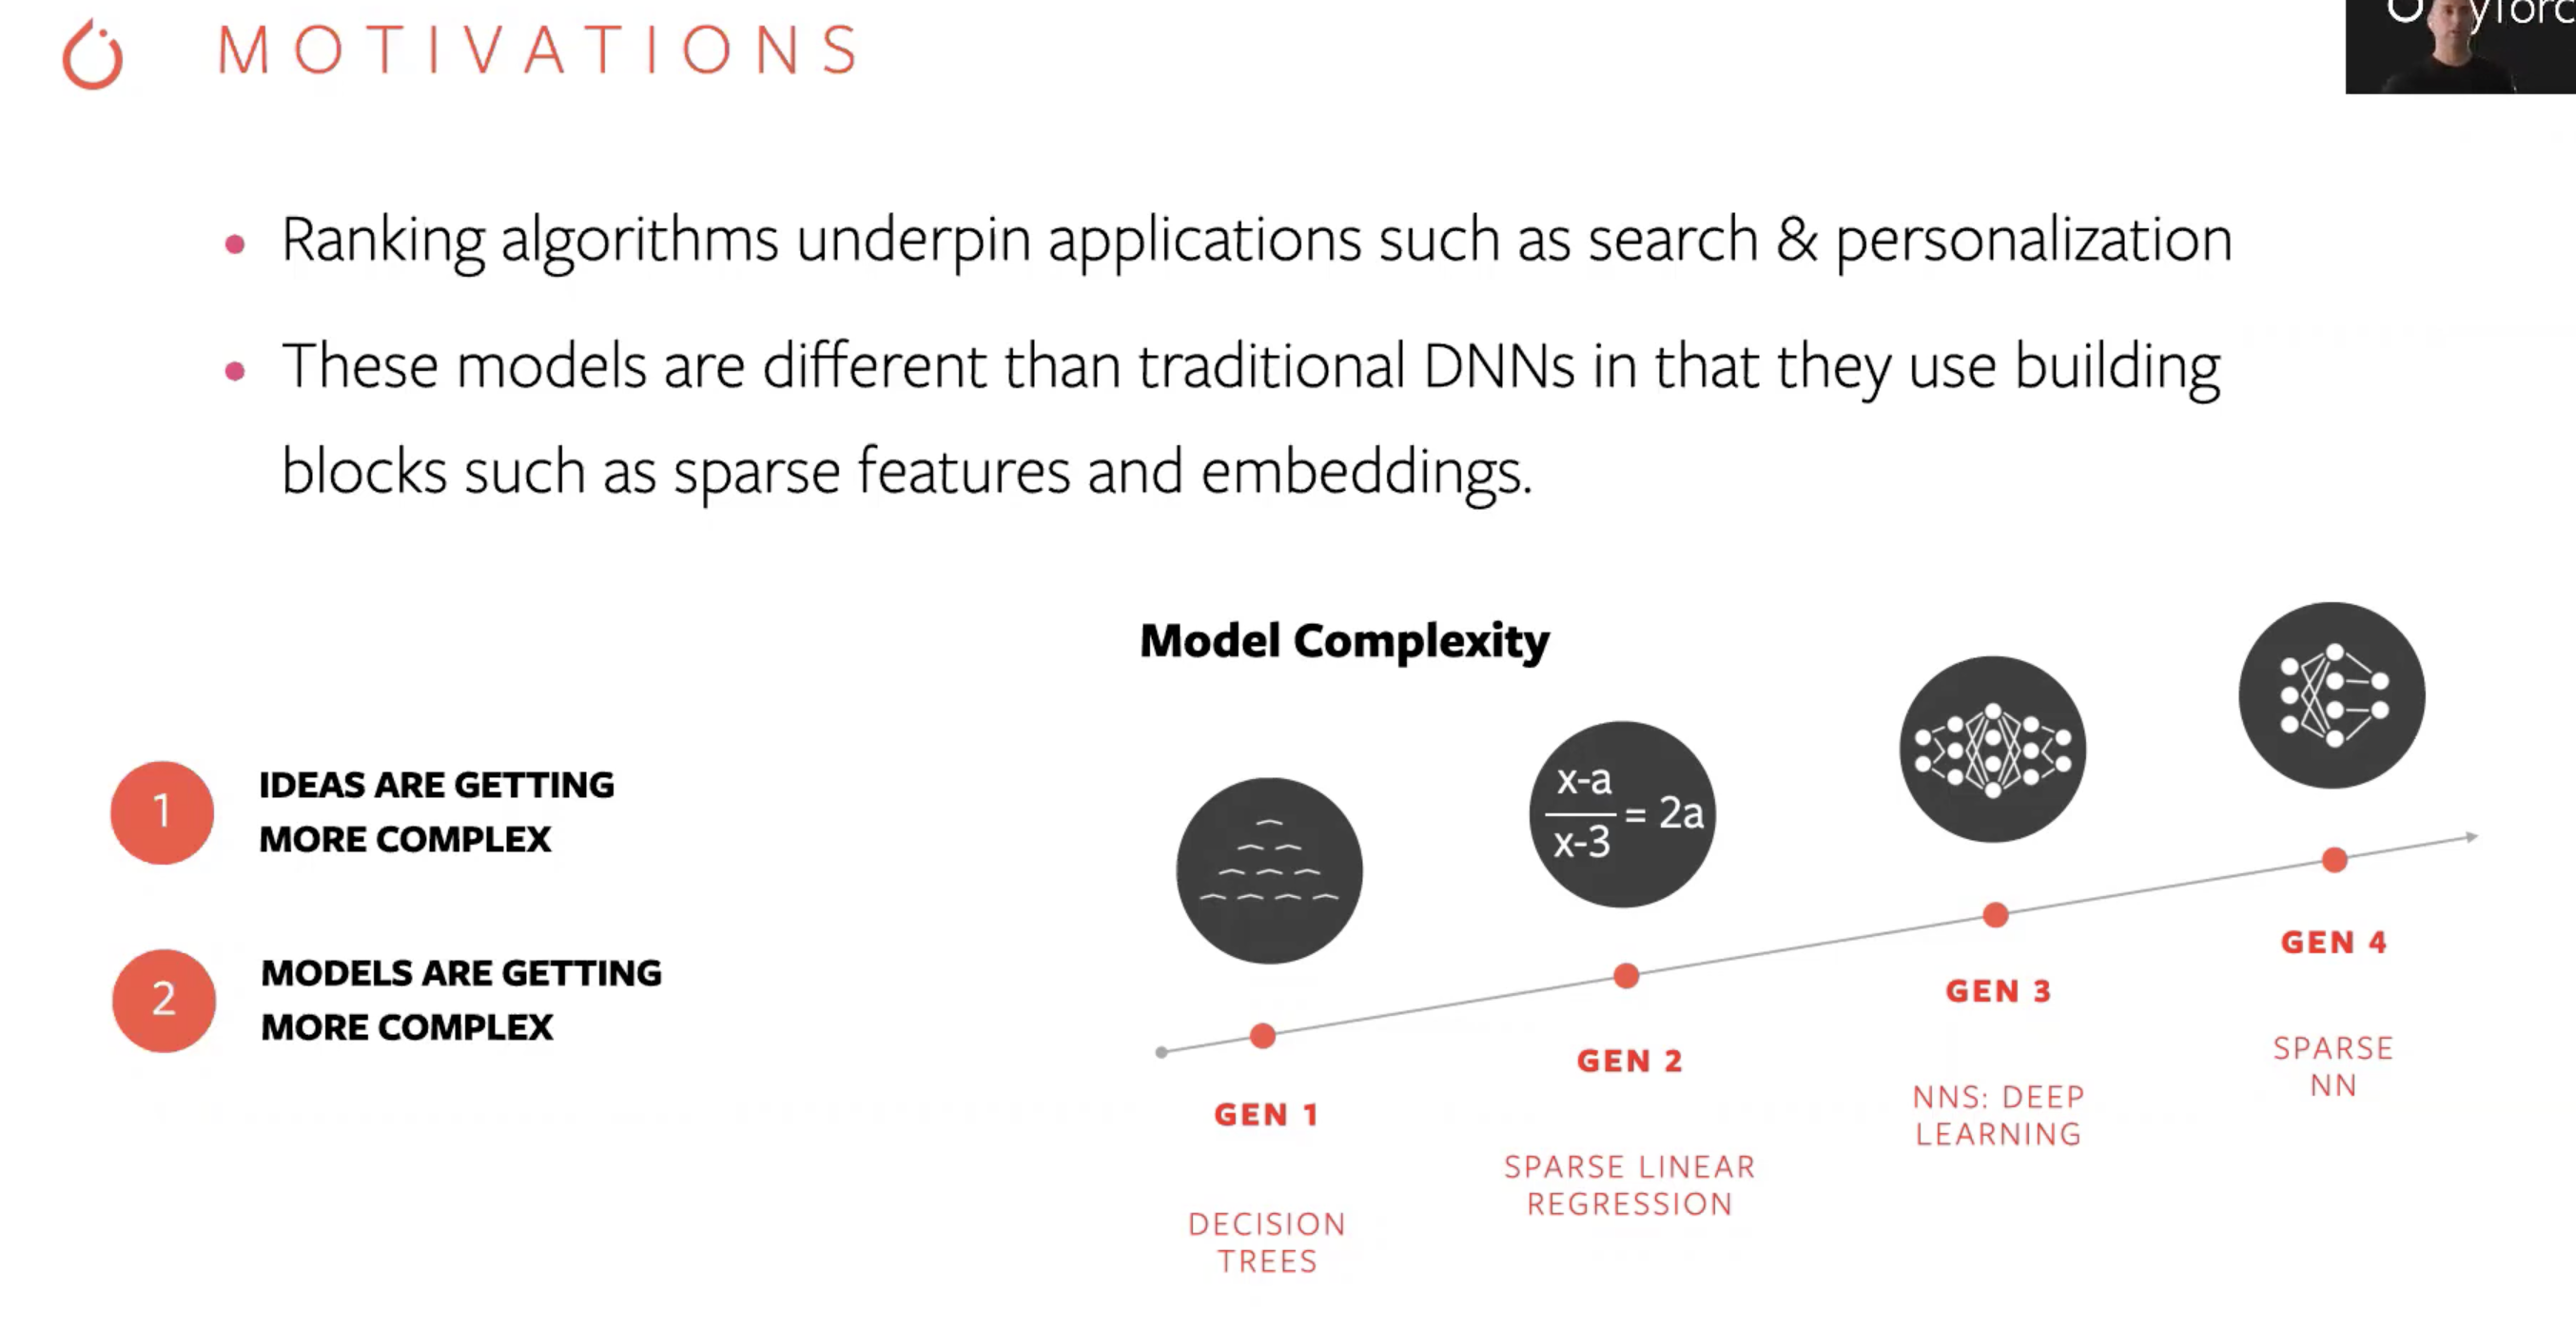
\includegraphics[width=0.8\linewidth]{parts/recsys/images/dlrm.png}
        \end{figure}
        
        Также полезные ссылки: Microsoft Recommenders (\url{https://arxiv.org/pdf/2008.13528.pdf}), NVIDIA Merling (\url{https://github.com/NVIDIA/HugeCTR})
    \item Немного про Captum - библиотека для интерпретации самых разных PyTorch моделей (например, выделение важных частей в инпуте) работающих с самыми разными входными данными (табличные, текст, картинки) --- \url{https://www.youtube.com/watch?v=fzrq1QGwsVo&feature=emb_logo}
        \begin{figure}[ht]
            \centering
            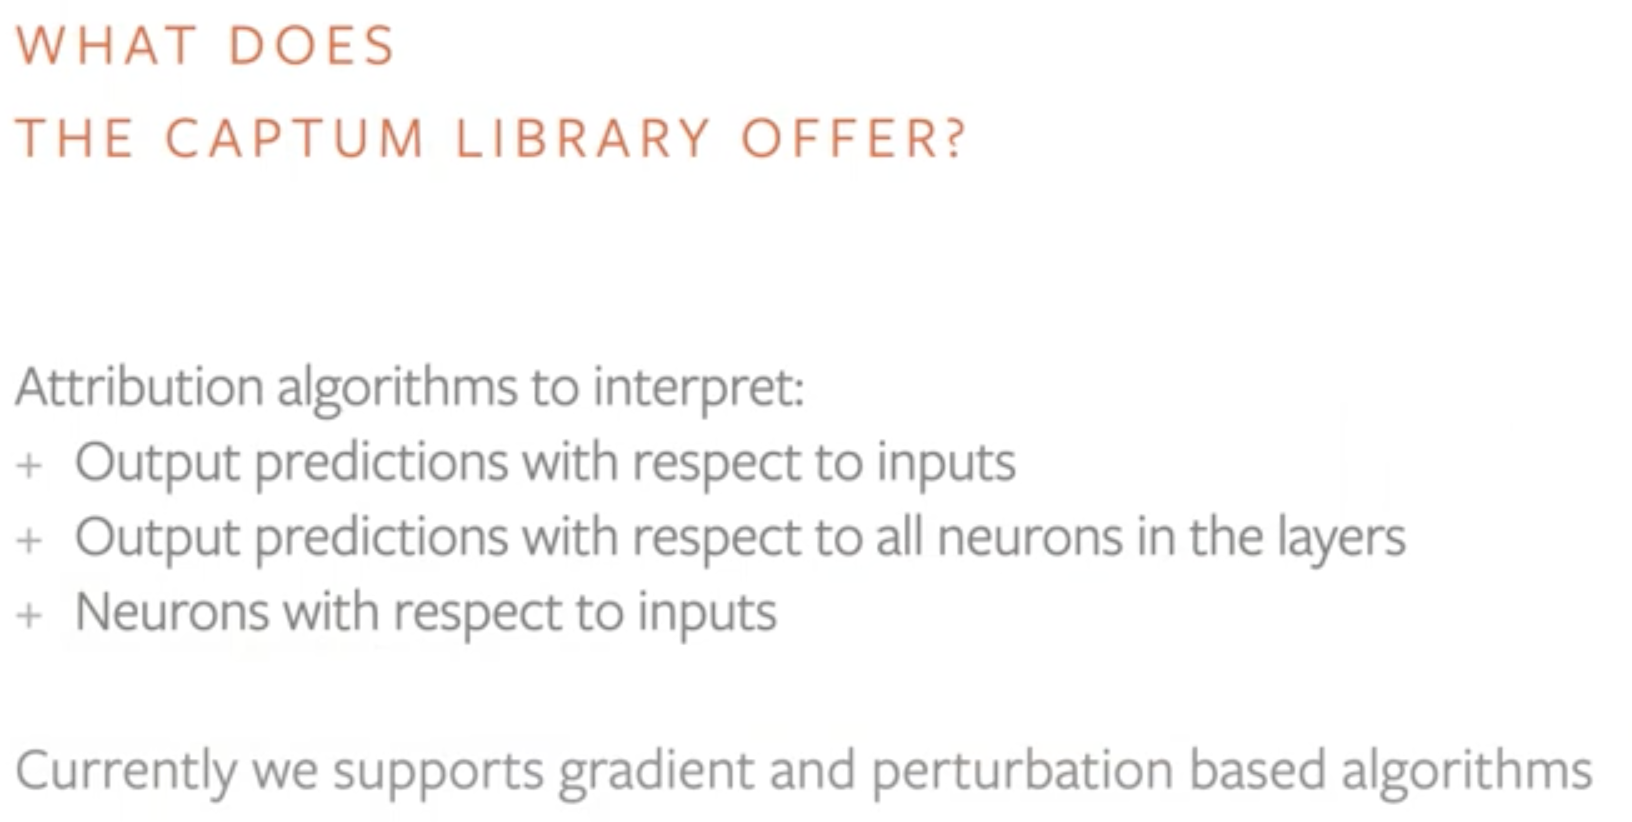
\includegraphics[width=0.5\linewidth]{parts/recsys/images/captum.png}
        \end{figure}
    \item Hands On: MMF фрэймворк для обучения моделей, которые на вход получают картинки И текст (например Visual Question Answering) --- \url{https://www.youtube.com/watch?v=quNtfWwNmPw&feature=emb_logo}
\end{enumerate}

% -----------------
% -- New Section --
% -----------------

\section*{[Linkedin] Image and Video Understanding for Recommendation and Spam Detection Systems}

Туториал состоит из двух больших частей - вводная часть и приложения в Linkedin.  

Вводную имеет смысл смотреть если хочется получить высокоуровневое представление о задачах и методах, которые возникают в Image and Video Understanding.

Самое интересное - приложения в Linkedin.

\paragraph{Вводная часть}

\begin{enumerate}
    \item Introduction to image and video usage in recommendations, search and spam detection at Linkedin --- \url{https://vimeo.com/445696336}
    \item Обзор основных задач связанных с \textbf{Image Understanding} - classification, segmentation, objects detection, captioning.
    
        Обзор методов получения представлений для изображений (с 10х годов и до наших дней) --- \url{https://vimeo.com/445696409}
    \item \textbf{Image representations} --- Кратко про NASNet (поиск архитектуры для ImageNet); EfficientNet (increase the efficiency, while maintaining accuracy) - very good choice if you are looking for a smaller network; Transfer Learning; Deep Metric Learning (siamese nets, contrastive loss); VilBERT --- \url{https://vimeo.com/445696505}
    \item \textbf{Video Understanding} --- Tasks (classification, segmentation, captioning)  --- \url{https://vimeo.com/445696678}
    \item Video Understanding - \textbf{Temporal Deep Learning Methods} --- \url{https://vimeo.com/445696755}, \url{https://vimeo.com/445696881}
    \item Video applications for \textbf{speech recognition} --- обзор современных и не очень методов --- \url{https://vimeo.com/445696966}
\end{enumerate}

\paragraph{Applications at Linkedin}

\begin{enumerate}
    \item Кратко про \textbf{пайплайны} (оффлайн/онлайн части) связанные с обработкой изображений и видео. \textbf{Video Search} - speech-to-text --- \url{https://vimeo.com/445697241}
    \item \textbf{Feed and Ads Modeling} --- чуть подробнее о том, как получают эмбеддинги для видео (коллаборативные и не очень) --- \url{https://vimeo.com/445697405}
    \item \textbf{Feed and Ads} --- Member Video Affinity (предсказание вероятности взаимодействия пользователя с видео) as a feature in Ranking Model --- \url{https://vimeo.com/445697492}
    \item \textbf{Spam Detection} --- пайплайны и модели --- \url{https://vimeo.com/445697551}
\end{enumerate}

% -----------------
% -- New Section --
% -----------------

\section*{[Amazon] Practical AutoML for Tabular, Text, and Image Data}

\textbf{Link:}~\url{https://jwmueller.github.io/KDD20-tutorial/} \\

Туториал

% -----------------
% -- New Section --
% -----------------

\section*{[Microsoft] AutoML}
\textbf{Video:}~\url{https://www.youtube.com/watch?time_continue=537&v=OoNeBuXkLeg&feature=emb_logo} \\

Microsoft Azure AutoML Platform from a user point of view.

% -----------------
% -- New Section --
% -----------------

\section*{Reinforcement Learning}

Всякое разное про современный RL \\

\url{https://www.youtube.com/watch?v=-Y6fmyMWIQ0}

\url{https://www.youtube.com/watch?time_continue=3&v=mLT3AgrOSsQ&feature=emb_logo}

\url{https://www.youtube.com/watch?time_continue=3&v=LIKrJnCo5fY&feature=emb_logo}

% -----------------
% -- New Section --
% -----------------

\section*{Robust Deep Learning Methods for Anomaly Detection} 

\textbf{Link:}~\url{https://github.com/raghavchalapathy/KDD-Tutorials-2020-Deep-Robust-Anomaly-Detection} \\

Использование автоэнкодеров для решения задачи детекции аномалий. 

\paragraph{Videos}

\begin{enumerate}
    \item Настройка окружения в Google Colab --- \url{https://www.youtube.com/watch?time_continue=4&v=8TY1UHYcjzk&feature=emb_logo}, \url{https://www.youtube.com/watch?v=H0t09clEkU4&feature=emb_logo}
    \item Обзор всяких разных Autoencoder'ов (AE, VAE, Adversarial AE, Wasserstein AE), введение в использование AE для anomaly detection --- \url{https://www.youtube.com/watch?v=UdWTRdhIdQY&feature=emb_logo}
    \item Hands On: AE for anomaly detection with toy dataset (Keras) --- \url{https://www.youtube.com/watch?v=BF3Plbp08sQ&feature=emb_logo}
    \item Introduction to Robust (Convolutional) AE --- \url{https://www.youtube.com/watch?v=unkue4h5f4A&feature=emb_logo}
    \item Hands On: RAE implementation --- \url{https://www.youtube.com/watch?v=rp1Z7DVt_ZA&feature=emb_logo}
\end{enumerate}

% -----------------
% -- New Section --
% -----------------

\section*{How to Calibrate Your Neural Network Classifier}

\textbf{Link:}~\url{https://github.com/nplan-io/kdd2020-calibration}

\textbf{Video:}~\url{https://www.youtube.com/watch?v=I4jikv07DFw&feature=emb_logo}

\textbf{Основная статья:}~\url{https://arxiv.org/pdf/1706.04599.pdf}

\paragraph{О чем туториал}

\begin{itemize}
    \item Что такое калибрация и зачем она нужна
    \item Reliability diagram\footnote{\url{https://towardsdatascience.com/introduction-to-reliability-diagrams-for-probability-calibration-ed785b3f5d44}} - как инструмент для проверки калибрации модели; Expected/Maximum Calibration Error - численный способ оценить калибрацию модели
    \item Calibration for multi-class case
    \item Calibration Methods --- isotonic regression, Platt scaling, temperature scaling
\end{itemize}

Туториал содержит как теоретическую часть так и code sessions.